%%%%%%%%%%%%%%%%%%%%%%%%%%%%%%%%%%%%%%%%
%% Local basis functions in 1D and 2D %%
%%%%%%%%%%%%%%%%%%%%%%%%%%%%%%%%%%%%%%%%

\chapter{Local Shape Functions and its Gradients} \label{chap:shap_fct} \index{shape functions|(} \index{basis functions|see{shape functions}} \index{gradients of shape functions|see{shape functions}}

 Assume we have already given or generated a mesh. The task is to find a basis of locally supported functions for the finite dimensional vector space $V_N$ (of certain polynomials) s.t. the basis functions are associated to a single cell/edge/face/vertex of the mesh and that the supports are the closure of the cells associated to that cell/edge/face/vertex. \\

 Once we have given the shape functions we can then continue to calculate the stiffness and mass matrices as well as the load vectors. \\

 By restricting global shape functions to an element of the mesh we obtain the local shape functions. They are computed on one of the following standard reference elements: intervals $[0,1]$ or $[-1,1]$, triangles with vertices $(0,0)$, $(1,0)$ and $(0,1)$ or squares $[0,1]^2$. If not stated otherwise the dimension is two and the functions are real-valued. \\

 Different methods are implemented in LehrFEM, stored in the folder \linebreak
 {\tt /Lib/Elements} and described in the following. For some shape functions you can run the scripts in the folder {\tt /Examples/PlotShap} to see the plots. %, or generally have a look at the finite element solvers in {\tt /Examples}. \\


%%%%%%%%%%%%%%%%%%%%%%%%%%%%%%%%
%% Input and Output Arguments %%
%%%%%%%%%%%%%%%%%%%%%%%%%%%%%%%%

\section{Input and Output Arguments}

 Throughout {\tt shap} was used for 'shape functions' and these programs compute the values of the shape functions for certain finite elements at the $Q$ quadrature points {\tt x} of the standard reference elements. The details for the input may be found in table \ref{tab:shap_in}.

\begin{table}[htb]
  \begin{tabular}{p{0.5cm}p{10.5cm}}
	{\tt x} & {\small $Q$-by-$1$ (1D) or $Q$-by-$2$ (2D) matrix specifying all quadrature points} \\
    	{\tt p} & {\small nonnegative integer which specifies the highest polynomial degree (only needed for Legendre and $hp$ polynomials, cf. \ref{ssect:shap_Leg} and \ref{ssect:shap_hp})}
  \end{tabular}
  \caption{Argument list for {\tt shap}- and {\tt grad\_shap}-functions\index{shape functions!argument list}}
  \label{tab:shap_in}
\end{table}

 The file name {\tt grad\_shap} stands for 'gradient of shape functions' respectively. If not specified otherwise both functions are for example called by \\

\noindent {\tt >> shap = \ttindex{shap\_LFE}(x);} \\
\noindent {\tt >> grad\_shap = \ttindex{grad\_shap\_LFE}(x);} \\

 The output in the real-valued case can be found in table \ref{tab:shap_out}. In the vectorial case every two subsequent columns form one $2$-dimensional shape function, hence the matrix contains twice as many columns. The number of shape functions per element depends on the local degrees of freedom ($l$).

\begin{table}[htb]
  \begin{tabular}{p{2cm}p{9cm}}
	{\tt shap} & {\small $Q$-by-$l$ matrix which contains the computed values of the shape functions at the quadrature points {\tt x}.} \\
	{\tt grad\_shap} & {\small $Q$-by-$2l$ matrix which contains the values of the gradients of the shape functions at {\tt x}. Here the ($2i-1$)-th column represents the $x_1$-derivative resp. the $2i$-th column the $x_2$-derivative of the $i$-th shape function.}
  \end{tabular}
  \caption{Output of {\tt shap}- and {\tt grad\_shap}-functions (real-valued)\index{shape functions!output}}
  \label{tab:shap_out}
\end{table}

 Before we start to discuss the different basis functions, the 3D plotting routines are desribed.


%%%%%%%%%%%%%%%%%%%%%%%%%%%%%%%
%% Plots  of shape functions %%
%%%%%%%%%%%%%%%%%%%%%%%%%%%%%%%

\section{Plotting Shape Functions} \label{sect:shap_plot} \index{shape functions!plot|(} \index{plot!shape functions|(}

 The function \ttitindex{plot\_Shap} stored in {\tt /Lib/Plots} generates a 3D plot with lighting effect of {\tt U} on the domain represented by {\tt Vertex}. It is called by \\

\noindent {\tt >> H = plot\_Shap(Vertex,U);} \\

 and returs the handle {\tt H} to the figure. \\

 As already mentioned, most implemented shape functions may be plotted using the plotting routines in the folder {\tt /Examples/PlotShap}. Their functions name is of the form {\tt main\_Shap\_*} where {\tt *} is replaced by the respective finite element. They make use of the function {\tt plot\_Shap} and the respective shape function {\tt shap\_*}. The 3 linear shape functions on the reference triangle are e.g. plotted by \\

\noindent {\tt >> \ttindex{main\_Shap\_LFE};} \\

 Furthermore, the function {\tt plot\_Shap} is applied to linear resp. quadratic basis functions in \ttitindex{plot\_Shap\_LFE}\index{linear finite elements!shape functions} and \ttitindex{plot\_Shap\_QFE}\index{quadratic finite elements!shape functions} (both stored in {\tt /Lib/Plots}) which generate 3D plots of the shape functions in \ttindex{shap\_LFE} resp. \ttindex{shap\_QFE} on the domain represented by {\tt Vertex}. They are e.g. called by \\

\noindent {\tt >> H = plot\_Shap\_LFE(NMesh,LNumber,Vertex);} \\

 The input arguments are described in table \ref{tab:plot_shap_in}.

\begin{table}[htb]
  \begin{tabular}{p{2cm}p{9cm}}
    {\tt NMesh} & {\small number which determines how fine the mesh is} \\
    {\tt LNumber} & {\small integer from 1 to 3 (resp. 1 to 6) that determines which {\tt LFE} (resp. {\tt QFE}) shape function to take} \\
    {\tt Vertex} & {\small matrix which determines the set of point which represent the domain of plotting}
  \end{tabular}
  \caption{Input for {\tt plot\_Shap}-routines}
  \label{tab:plot_shap_in}
\end{table}

 
 Figure \ref{fig:plot_Shap} shows the output for {\tt plot\_Shap\_LFE} and {\tt plot\_Shap\_QFE} on the unit triangle for first linear resp. quadratic shape function , cf. \ref{sssect:shap_LFE}. {\tt NMesh} was set to $100$, {\tt LNumber} is $1$. \\

\begin{figure}[htb]
  \centering
  \begin{minipage}[c]{0.8\textwidth}
    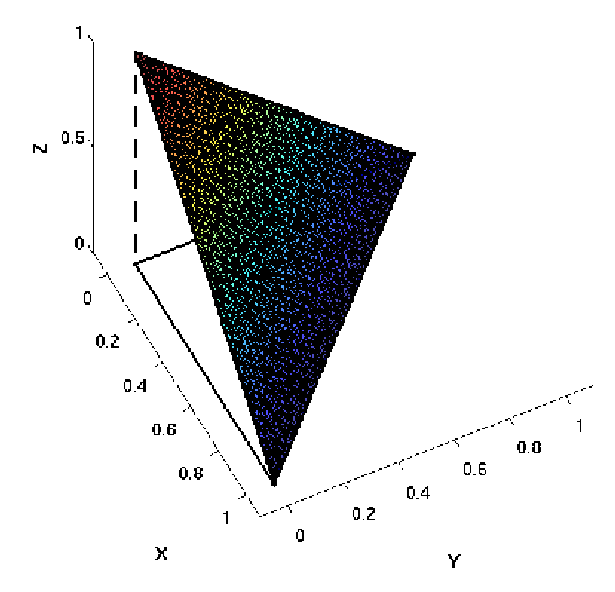
\includegraphics[width=0.4\textwidth]{plot_Shap_LFE.eps} \hfill
    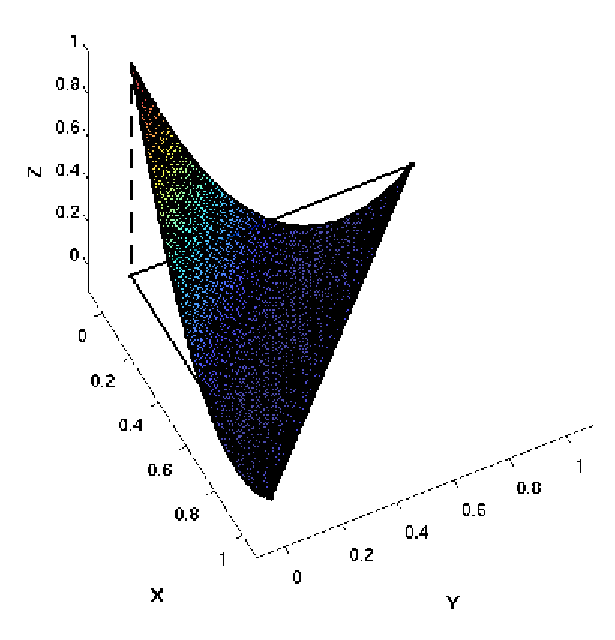
\includegraphics[width=0.4\textwidth]{plot_Shap_QFE.eps}
  \end{minipage}
  \caption{Output of {\tt plot\_Shap\_LFE} and {\tt plot\_Shap\_QFE}}
  \label{fig:plot_Shap}
\end{figure}

 In the above functions \ttitindex{affine\_map} is used to generate a mapping of all the vertices in the struct {\tt Mesh} (resp. {\tt Coordinates} in 1D) by the mapping from the reference element to the element which is formed by the given {\tt Vertices} in row-wise orientation. It is called by one of the following lines. \\

\noindent {\tt >> Coordinates = affine\_map(Coordinates,Vertices);} \\
\noindent {\tt >> Mesh = affine\_map(Mesh,Vertices);} \\


\subsection{Pyramid Plots} \index{shape functions!plot pyramids}

 For linear and quadratic finite elements it's also possible to plot the global shape functions by combination of the local shape functions. These routines are named {\tt plot\_Pyramid\_*} and stored in the folder {\tt /Examples/PlotShap}. They make use of the above {\tt plot\_Shap}-function and are e.g. called by \\

\noindent {\tt >> \ttindex{plot\_Pyramid\_LFE};} \\

 See figure \ref{fig:plot_pyramid} for the output of \ttindex{plot\_Pyramid\_LFE} and \ttindex{plot\_Pyramid\_QFE} and compare them to figure \ref{fig:plot_Shap}.

\begin{figure}[htb]
  \centering
  \begin{minipage}[c]{0.8\textwidth}
    \includegraphics[width=0.4\textwidth]{Shap_Pyramid3D_LFE.eps} \hfill
    \includegraphics[width=0.4\textwidth]{Shap_Pyramid3D_QFE.eps}
  \end{minipage}
  \caption{Output of {\tt plot\_Pyramid\_LFE} and {\tt plot\_Pyramid\_QFE}}
  \label{fig:plot_pyramid}
\end{figure}

\index{plot!shape functions|)}
\index{shape functions!plot|)}


%%%%%%%%%%%%%%%%%%%%%%%%%%%%%%%
%% Different shape functions %%
%%%%%%%%%%%%%%%%%%%%%%%%%%%%%%%

\section{Different Shape Functions} \label{sect:shap}


%%% Lagrangian finite elements %%%

\subsection{Lagrangian Finite Elements}


\subsubsection{of order 1, $H^1$-conforming} \index{shape functions!Lagrangian finite elements!of order 1!conforming} \index{linear finite elements!shape functions|(} \label{sssect:shap_LFE}

 The function \ttitindex{shap\_LFE} is used to compute the values of the three shape functions and \ttitindex{grad\_shap\_LFE} for the gradients for triangular Lagrangian finite elements. \\

 These shape functions may be plotted using \ttitindex{main\_Shap\_LFE} in \linebreak
 {\tt /Examples/PlotShap} or \ttindex{plot\_Shap\_LFE} in {\tt /Lib/Plots}. The pyramid is generated by \ttitindex{plot\_Pyramid\_LFE} in {\tt /Examples/PlotShap}. See the left figures in \ref{fig:plot_Shap} and \ref{fig:plot_pyramid}.


\subsubsection{of order 1, vector-valued} \index{shape functions!Lagrangian finite elements!of order 1!vector-valued} \index{linear vector-valued finite elements!shape functions}

 \ttitindex{shap\_LFE2} is also of order 1 but vector-valued, hence the functions are the same as in {\tt shap\_LFE} (in one coordinate, the other one is $0$). In the output every two columns belong together and form one 2-dimensional shape function. They can be plotted on the reference triangle using the following command from the folder {\tt /Examples/PlotShap}

\noindent {\tt >> \ttindex{plot\_Shap\_LFE2};} \\

% These functions are not conforming. For conforming vector-valued shape functions see \ref{ssect:shap_W1F}.


\subsubsection{of order 2, conforming} \label{sssect:shap_QFE} \index{quadratic finite elements!shape functions}

 \ttitindex{shap\_QFE} and \ttitindex{grad\_shap\_QFE} compute the values of the shape functions resp. gradients of the functions for triangular Langrangian finite elements. In \linebreak {\tt shap\_QFE} the first three columns are the shape functions supported on vertices and the last three columns the ones supported on edges. \\

 These shape functions may be plotted using \ttitindex{main\_Shap\_QFE} in \linebreak
 {\tt /Examples/PlotShap} or \ttindex{plog\_Shap\_QFE} in {\tt /Lib/Plots}. The pyramid is generated by \ttitindex{plot\_Pyramid\_QFE} in {\tt /Examples/PlotShap}. See figures on the right hand side in \ref{fig:plot_Shap} and \ref{fig:plot_pyramid}. \\

 \ttitindex{shap\_EP2} and \ttitindex{grad\_shap\_EP2} compute the values of the functions resp. gradients of the functions for triangular Langragian finite elements connected to edges. As mentioned above these functions are also contained in {\tt shap\_QFE} and {\tt grad\_shap\_QFE}, but in a different order. \\

These shape functions of order 1 and 2 are e.g. used for the Stokes problem.


\subsubsection{Discontinuous Linear Lagrangian Finite Element in 1D ..} 

 \ttitindex{shap\_DGLFE\_1D} and \ttitindex{grad\_shap\_DGLFE\_1D} compute the values of the shape functions resp. its gradients for {\tt x}$\in [-1,1]$.


\subsubsection{.. and 2D}

 \ttitindex{shap\_DGLFE} and \ttitindex{grad\_shap\_DGLFE} are actually the same functions as {\tt shap\_LFE} and {\tt grad\_shap\_LFE}. \\ 

 They are used in the discontinuous Galerkin method.


\subsubsection{Linear Finite Elements (1D)} \label{sssect:shap_P1_1D} 

 \ttitindex{shap\_P1\_1D} computes the values of the two linear shape functions in one dimension where {\tt x} are points in the interval $[0,1]$. The first column {\tt shap(:,1)} is \texttt{1-x} and {\tt shap(:,2)} is \texttt{x}. \\

 \ttitindex{grad\_shap\_P1\_1D} computes the gradients \texttt{-1} and \texttt{1} respectively.

\index{linear finite elements!shape functions|)}


\subsubsection{Bilinear Finite Elements} \label{sssect:shap_BFE} \index{bilinear finite elements!shape functions}

 \ttitindex{shap\_BFE} computes the values of the four bilinear shape functions at \texttt{x}$\in [0,1]^2$, \ttitindex{grad\_shap\_BFE} the partial derivatives. The bilinear shape functions may be plotted using \ttitindex{main\_Shap\_BFE} in {\tt /Examples/PlotShap}.


\subsubsection{Crouzeix-Raviart Finite Elements} \index{Crouzeix-Raviart finite elements!shape functions}

 \ttitindex{shap\_CR} and \ttitindex{grad\_shap\_CR} compute the shape functions resp. its gradients for the Crouzeix-Raviart finite element at the quadrature points \texttt{x} of a triangle. %with vertices $(0,0)$, $(1,0)$ and $(0,1)$.
 Unlike the conforming shape functions the Crouzeix-Raviart finite elements are $0$ at the midpoints of two edges and $1$ at the opposite midpoint. \\

 The Crouzeix-Raviart shape functions may be plotted using \ttitindex{main\_Shap\_CR} in {\tt /Examples/PlotShap}. \\

 \ttitindex{shap\_DGCR} and \ttitindex{grad\_shap\_DGCR} do the same for the discontinuous case. The Crouzeix-Raviart finite elements are e.g. used for the discontinuous Galerkin method and the Stokes problem.


%%% MINI element %%%

\subsection{MINI Element} \index{MINI element!shape functions}

 \ttitindex{shap\_MINI} computes the values of four shape functions for the triangular MINI element, \ttitindex{grad\_shap\_MINI} its gradients. The first three columns are the linear elements, the fourth one is the element shape function which is $0$ on the edges and $1$ in the center, also referred to as 'bubble function'.


%%% Whitney 1-forms %%%

\subsection{Whitney 1-Forms} \label{ssect:shap_W1F} \index{Whitney 1-forms!shape functions} \index{edge elements|see{Whitney 1-forms}}

Similar to {\tt shap\_LFE2} the Whitney 1-forms \ttitindex{shap\_W1F} are vector-valued and two columns together form one function. Whitney forms are finite elements for differential forms. The 1-forms are edge elements and $H(curl)$-conforming. See e.g. \cite{MO03} for more details. For plotting the shape functions on the reference triangle use \\ 

\noindent {\tt >> \ttindex{plot\_Shap\_W1F};} \\

which can be fount in the {\tt /Examples/PlotShap} folder.


% \textcolor{pink}{The degrees of freedom are integrals. The Whitney 1-forms are tangentially continous.}


%%% Legendre polynomials %%%

\subsection{Legendre Polynomials up to degree {\tt p}} \label{ssect:shap_Leg}

 \ttitindex{shap\_Leg\_1D} computes the values of the Legendre polynomials up to degree {\tt p}, used as shape functions for the 1D $hp$DG discretizations. They are called by \\

\noindent {\tt >> shap = shap\_Leg\_1D(x,p);} \\

 with {\tt x}$\in [-1,1]$ and {\tt p}$\geq 0$. %They are computed using an recursion.
 The ({\tt n+1})-th column {\tt shap(:,n+1)} in the output is the Legendre polynomial of degree {\tt n} at {\tt x}.\\

\ttitindex{grad\_shap\_Leg\_1D} computes the gradients analogously.


%%% Hierarchical shape functions %%%

\subsection{Hierarchical Shape Functions up to polynomial degree {\tt p}} \label{ssect:shap_hp} \index{hpFEM@$hp$FEM!shape functions}

 \ttitindex{shap\_hp} computes the values and gradients of the hierarchical shape functions on the reference element up to polynomial degree {\tt p} at the points {\tt x}. It is called by \\

\noindent {\tt >> shap = shap\_hp(x,p);} \\

 Vertex, edge and element shape functions are computed. If {\tt i} is the number of the vertex/edge, then the associated polynomials of degree {\tt p} and its gradients are called by \\

\noindent {\tt >> shap.vshap$\left\lbrace \texttt{i} \right\rbrace$.$\left\lbrace \texttt{p} \right\rbrace$;} \\
\noindent {\tt >> shap.vshap$\left\lbrace \texttt{i} \right\rbrace$.grad\_shap$\left\lbrace \texttt{p} \right\rbrace$;} \\
\noindent {\tt >> shap.eshap$\left\lbrace \texttt{i} \right\rbrace$.shap$\left\lbrace \texttt{p} \right\rbrace$;} \\
\noindent {\tt >> shap.eshap$\left\lbrace \texttt{i} \right\rbrace$.grad\_shap$\left\lbrace \texttt{p} \right\rbrace$;} \\
\noindent {\tt >> shap.cshap.shap$\left\lbrace \texttt{p} \right\rbrace$;} \\
\noindent {\tt >> shap.cshap.grad\_shap$\left\lbrace \texttt{p} \right\rbrace$;} \\

 where \ttitindex{vshap} stands for vertex shape function, \ttitindex{eshap} for edge and \ttitindex{cshap} for element shape function respectively. \\

 This program is part of the $hp$FEM. They are called hierarchical shape functions because when enriching from order {\tt p} to {\tt p+1} the existing shape functions don't change, but new ones are added. See \cite{AI03} for more information. \\

 The hierarchical shape functions may be plotted using \ttitindex{main\_Shap\_hp} in {\tt /Examples/PlotShap}.

\index{shape functions|)}